\documentclass[a4paper]{article}

\usepackage{graphicx}
\usepackage{amsmath}
\usepackage{multirow}
\usepackage[bottom=2cm, right=1.5cm, left=1.5cm, top=1.5cm]{geometry}\usepackage{rotating}
\usepackage{longtable}
\usepackage{booktabs}
\usepackage{mathtools}
\usepackage{hhline}
\usepackage[pdfauthor={Alexandre S. Avaro},pdftitle={Image processing of bead images using MATLAB}]{hyperref}
\usepackage{float}
\usepackage{array}
\usepackage{textcomp}
\usepackage{libertine}
\usepackage[libertine]{newtxmath}
\usepackage{etoolbox}
\usepackage[T1]{fontenc}
\usepackage[utf8]{inputenc}
\usepackage{bm}

\begin{document}
\title{Image processing of bead images using MATLAB \\
\large{v0.1}}
\author{Alexandre S. Avaro, Pablo Ibáñez}
\maketitle

This document explains how to use the bead tracking and quantification tool based on MATLAB. This code uses image morphology tools to count beads and quantify signal in fluorescence microscopy images. 

\section{Requirements}
You will require the following to run the code:
\begin{itemize}
    \item A local MATLAB install. ESPCI provides a free MATLAB license to any user with an ESPCI email adress. See \href{https://www.mathworks.com/academia/tah-portal/espci-30728296.html}{here} to install MATLAB and get started.
    \item The code \verb|main.m| along with the helper function \verb|impaint_nans.m|. The codes are available directly \href{https://github.com/alexandre-avaro/bead-tracking}{here}.
    \item Epifluorescence images of the beads. The convention for this code is to store the images as \verb|.tif| files with one folder per conditions. Each condition folder contains the MATLAB codes, and one subfolder per fluorescence filter. By default, the code looks for folder denoted "Ftc" and "Cy5" (corresponding respectively to FITC and Cy5 epifluorescence images). Each subfolder contains the \verb|.tif| files with all the images corresponding to the same experimental condition and illumination.
\end{itemize}

\section{Getting started}
\subsection{Glossary}

\begin{tabular}{l|l}
    Condition & Set of images corresponding to the same experimental conditions. \\
    \hline
    Filter set & Set of images corresponding to the same illumination conditions \textbf{and} to the same experimental conditions. 
\end{tabular}

\subsection{Running the code}
To run the code, open \verb|main.m| in MATLAB and run the code. The code has to be run only once per condition to perform the analysis across all filter sets. The analysis may take a couple minutes (especially if there is a large number of images to analyze). If there is no error in the MATLAB console and all outputs files are created (see \ref{section-outputs}), the analysis has completed successfully.


\subsection{Outputs}
\label{section-outputs}
The tool gives the following outputs for each filter set Flt (typically, Flt = Ftc or Flt = Cy5):

\begin{itemize}
    \item Post-processed images [series of \verb|.tif| files]. These comprise two image sets:
    \begin{itemize}
        \item Background images: For each image, the tool extracts the background image (i.e., without beads). We detail how this background image is computed in section \ref{section-details}. Background images are stored in the "Flt/Bkg" folder.
        \item Treated images: Backgound-subtracted images. Treated images are stored in the "Flt/Trt" folder.
    \end{itemize}

    \item Histogram of the bead radii [one \verb|.png| file per filter set]. The calculation of the bead radius is detailed in section \ref{section-details}. Note that the bead detection is run for each filter set so the total number of beads $n_{\text{beads}}$ (indicated in the title of the plot) detected by the code may differ from one filter set to another. We indicate with a red line the median bead radius. The histogram is created in the folder where the MATLAB code is stored under the name \verb|Flt_comb_rad_hist.png|.
    \item Histogram of the bead integrated fluorescence intensity [one \verb|.png| file per filter set]. The calculation of the bead integrated intensity is detailed in section \ref{section-details}. Note that the bead detection is run for each filter set so the total number of beads $n_{\text{beads}}$ (indicated in the title of the plot) detected by the code may differ from one filter set to another. We indicate with a red line the median bead integrated intensity. The histogram is created in the folder where the MATLAB code is stored under the name \verb|Flt_comb_int_hist.png|.
    \item The list of bead radii and integrated intensities [one \verb|.csv| file per filter set], saved as \verb|Flt_rad_int.csv|.
\end{itemize}

Note that histogram outputs combine all the beads detected within one filter set, i.e. across multiple images.

\section{Detailed analysis process}
\label{section-details}
In this section, we detail the step-by-step image analysis pipeline that is run in this tool. The code examines subfolders contained within the folder where the code is stored and that are listed in the variable \verb|filter|. For each filter set Flt:

\begin{enumerate}
    \item Images are first loaded in the MATLAB workspace. Note that all TIF files in the folder "Flt" will be included in the analysis. Figure \ref{fig1} shows a typical raw bead image.
    \begin{figure}[H]
        \center
        \label{fig1}
        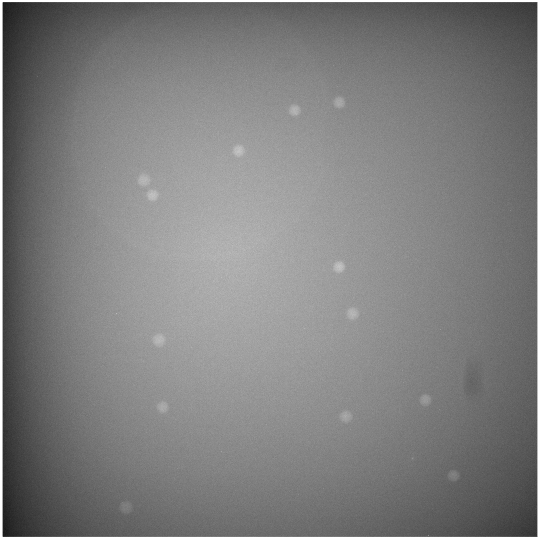
\includegraphics[scale=0.75]{im.png}
        \caption{Raw bead image}
    \end{figure}

    As you can see, the beads are visible but it is not easy to quantify clearly the fluorescence intensity of the beads this way. There is also significant vignetting in the image (i.e., the corners of the image are darker than the center). There are also background features that hinder the analysis of the beads (e.g., a very large disk in the center top of the image, or a smaller dark trace on the bottom right). We post-process these images to clean them up and quantify effectively the fluorescence on the beads.

    \item A binary mask is then created using the function \verb|imbinarize|. This function uses adaptive thresholding and outputs a binary image (i.e., composed of 0s and 1s). Here, "adaptive" is in opposition to "global" thresholding, in which each pixel intensity value is compared to a unique (= global) threshold. In adaptive thresholding, a local threshold is determined based on image statistics in the neighborhood of each pixel. Adaptive thresholding requires a sensitivity parameter set between 0 and 1. For the set of images used to develop this code, the optimal value of sensitivity was found to be 0.57. Figure \ref{fig2} shows the output of the \verb|imbinarize| function, using the image shown in figure \ref{fig1} as input.
    
    \begin{figure}[H]
        \center
        \label{fig2}
        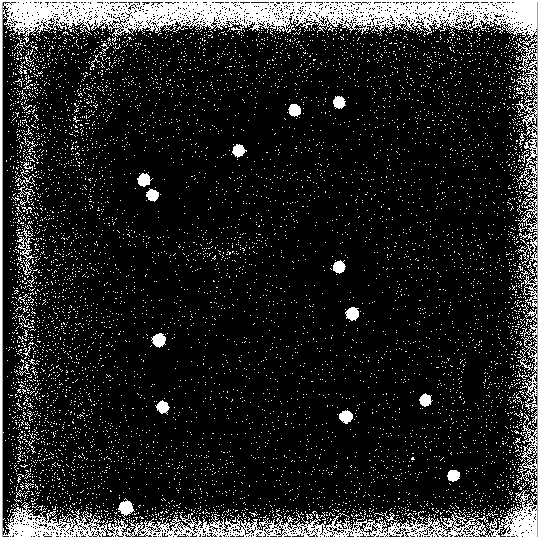
\includegraphics[scale=0.75]{firstbin.png}
        \caption{Binary image after adaptive binarization}
    \end{figure}

    The beads are clearly visible in this binary image as large regions of 1s (white), but there are a lot of speckled noise. These correspond to noise in the sensor yielding local maxima. 
    
    \item To get rid of the local noise, we proceed to an operation called "erosion". The erosion operation has two inputs: a binary image and an structuring element (i.e., a shape). It outputs a binary image. Each pixel with a 1 in the input image remains an 1 in the output image if and only if the structuring element centered at this pixel only touches pixels with 1s. Otherwise, it becomes a 0 in the output image. 
    
    Let us apply this simple yet powerful technique to our noisy image. We choose as a structuring element a disk that has a radius of 3 pixels (px). Most of the noisy pixels in our image (figure \ref{fig2}) are lone pixels surrounded by 0s. Therefore, if you place a disk that has a radius of 3 px (our structuring element) and set the center of the disk to be the noisy pixel, it will intersect with at least one 0 pixel. This will set the noisy pixel to 0. Conversely, the beads are contiguous packs of 1s, so they will be relatively unaffected by the operation. In MATLAB, the implementation is very simple using the functions \verb|strel| (to define a structuring element) and \verb|imerode| (to proceed to the erosion). Figure \ref{fig3} shows the result of the erosion.
    
    \begin{figure}[H]
        \center
        \label{fig3}
        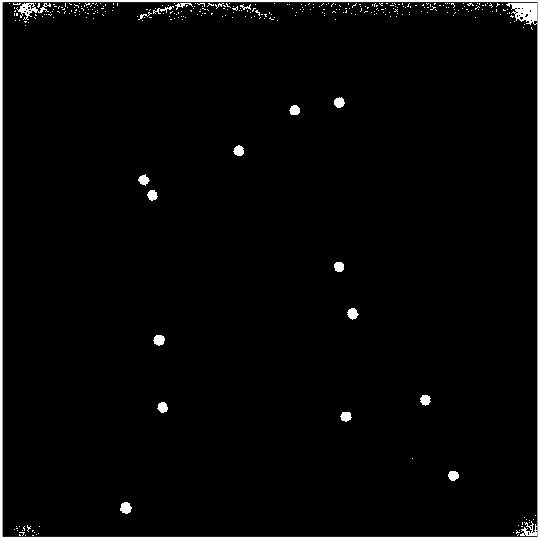
\includegraphics[scale=0.75]{firstbinerod.png}
        \caption{Binary image after erosion}
    \end{figure}

    As you can see, the erosion has enabled us to get rid of most of the noise. However, the pixels on the edge of the beads have been set to 0 by the erosion, which will induce an error in our estimation of the actual bead region. 
    
    \item To correct for this, we will apply the operation opposite to erosion: dilation. Similar to erosion, dilation uses a binary image and a struturing element. Then, all pixels that are in any region defined by a structuring element centered in a 1 pixel in the input image will be set to 1 in the output image. To correct for the erosion, we use the same structuring element in the dilation. Here, we again use a disk of radius 3 px. In MATLAB, this is done using the function \verb|imdilate|. Figure \ref{fig4} shows the result.
    
    \begin{figure}[H]
        \center
        \label{fig4}
        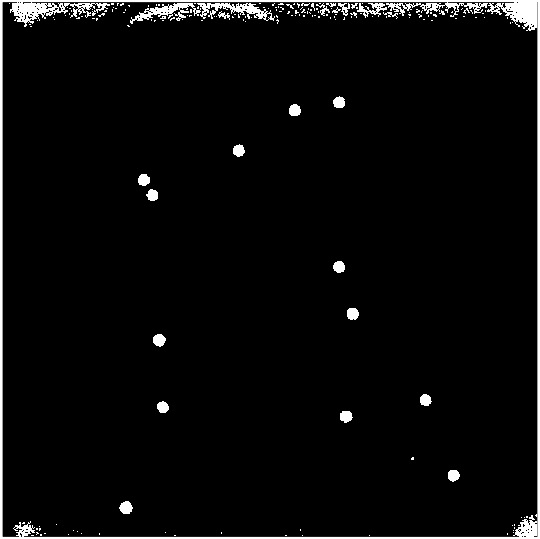
\includegraphics[scale=0.75]{bin.png}
        \caption{Binary image after dilation}
    \end{figure}

    Note that it is possible to run several rounds of erosion and dilation, with a wide variety of structuring elements (squares, lines, etc.). This results in the selection of some features over others, and could be optimized further.

    \item We now select the regions of interest for our analysis. Here, we know that, given the observation conditions (e.g., magnification), the beads should have a radius comprised between 12 and 30 pixels and that are (at least roughly) circular. MATLAB has a dedicated function to identify circular binary regions whose radius is in a given range: \verb|imfindcircles|. It outputs the position of the circles (in the form of $x$-$y$ coordinates) and radii. We then convert each circle to a circular binary region and create a new binary image using these regions only. Figure \ref{fig5} shows the resulting binary image.
    
    \begin{figure}[H]
        \center
        \label{fig5}
        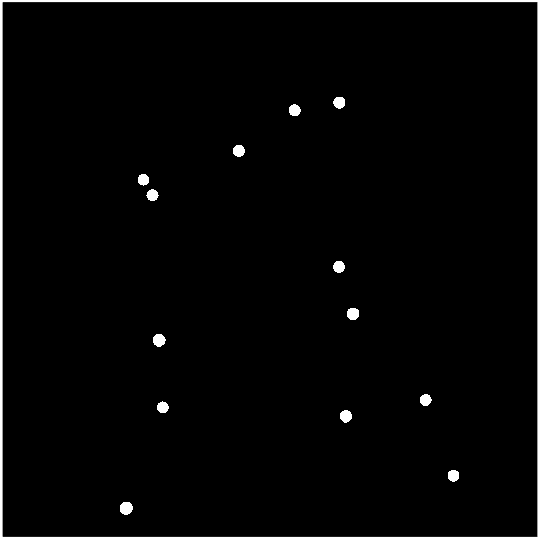
\includegraphics[scale=0.75]{circMask.png}
        \caption{Binary image after conservation of circular regions only}
    \end{figure}

    Note how this enabled to clean-up the background noise on top and bottom of the image. 
    
    \item We then remove any region that is touching the border of the image, so that we do not consider beads that are only partly imaged. Since there is no bead in this configuration here, the mask remains unchanged.
    \begin{figure}[H]
        \center
        \label{fig6}
        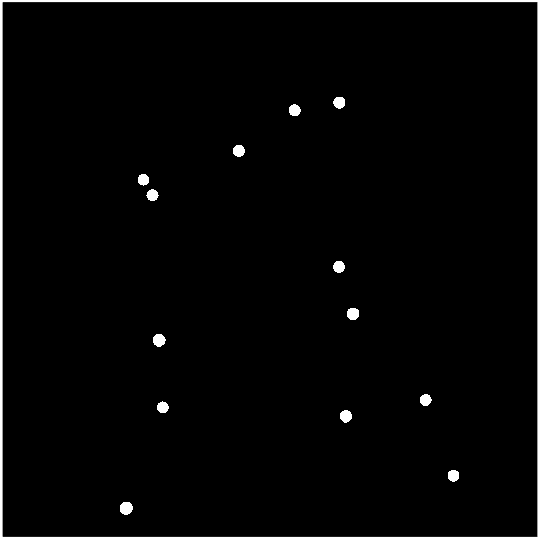
\includegraphics[scale=0.75]{cleanMask.png}
        \caption{Bead mask}
    \end{figure}

    We will use this binary image as a mask to compute the fluorescence intensities. You can think of this as a stencil where 1s are holes and 0s are filled.

    \item Before we go back to the original image, we will first define another mask with slightly larger "holes", so that we are safely away from the beads when we define what is signal from what is background in our image. To do that, we simply proceed to another dilation with a disk of radius 5 (to be safely away from the bead halo). We will call "background masks" images such as the one shown in figure \ref{fig7} and which result from this operation.
    \begin{figure}[H]
        \center
        \label{fig7}
        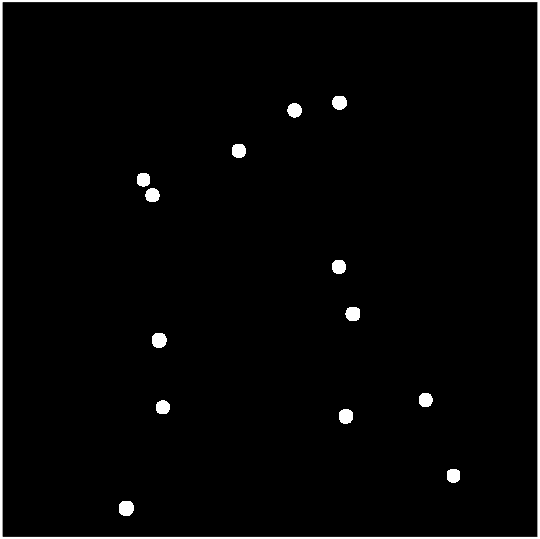
\includegraphics[scale=0.75]{cleanMaskbkg.png}
        \caption{Background mask}
    \end{figure}

    \item Let us now compute the background image. First, we will conserve from the original fluorescence image only the regions that are safely away from the beads. To this, we multiply the original image (figure \ref{fig1}) with the inverted background mask (figure \ref{fig7}). Figure \ref{fig8} shows the resulting image.
    \begin{figure}[H]
        \center
        \label{fig8}
        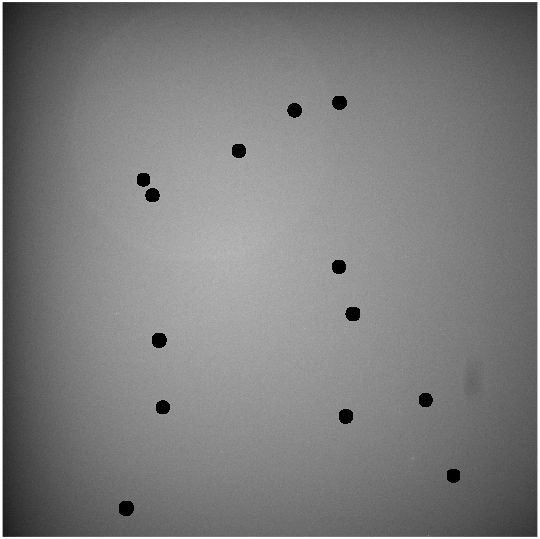
\includegraphics[scale=0.75]{bg.png}
        \caption{Fluorescence image multiplied by inverted background mask}
    \end{figure}

    \item We then interpolate the background image to reconstruct what the background would have been in the absence of the beads using the function \verb|impaint_nans.m|. This is a custom function developed by John D'Errico that replaces "NaN" pixels ("not a number") by a local interpolation. This code provides several interpolation methods. We here choose method 4 because it yields in the most satisfying results given the test images. Figure \ref{fig9} shows the following reconstructed background image.
    \begin{figure}[H]
        \center
        \label{fig9}
        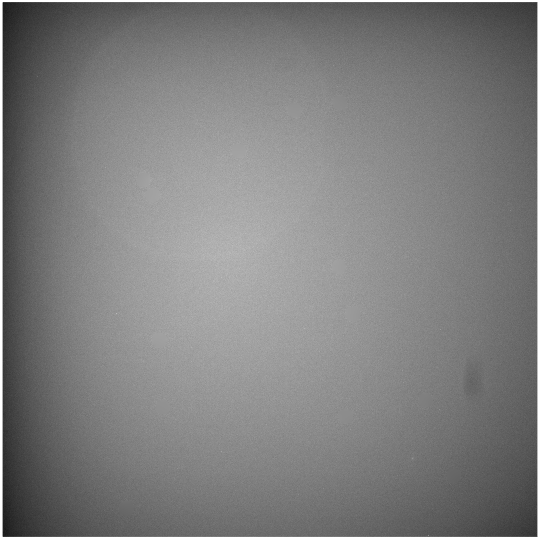
\includegraphics[scale=0.75]{bginterp.png}
        \caption{Reconstructed background image}
    \end{figure}
    This image is the background image that is saved and stored in the "Bkg" folder.

    \item We then compute the background-subtracted image by simply subtracting the reconstructed background image from the original image. Figure \ref{fig10} shows the final result.
    
    \begin{figure}[H]
        \center
        \label{fig10}
        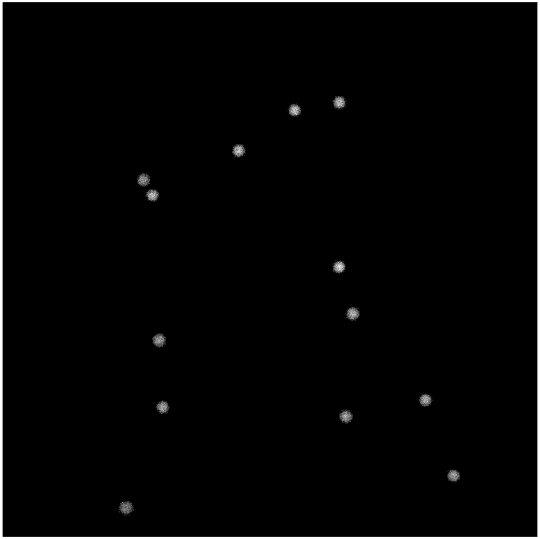
\includegraphics[scale=0.75]{treated.png}
        \caption{Treated image}
    \end{figure}

    This is the image that is saved and stored in the "Trt" folder. Figure \ref{fig11} shows the three saved images and example profile plot across the same sections for the three images.

    \begin{figure}[H]
            \center
            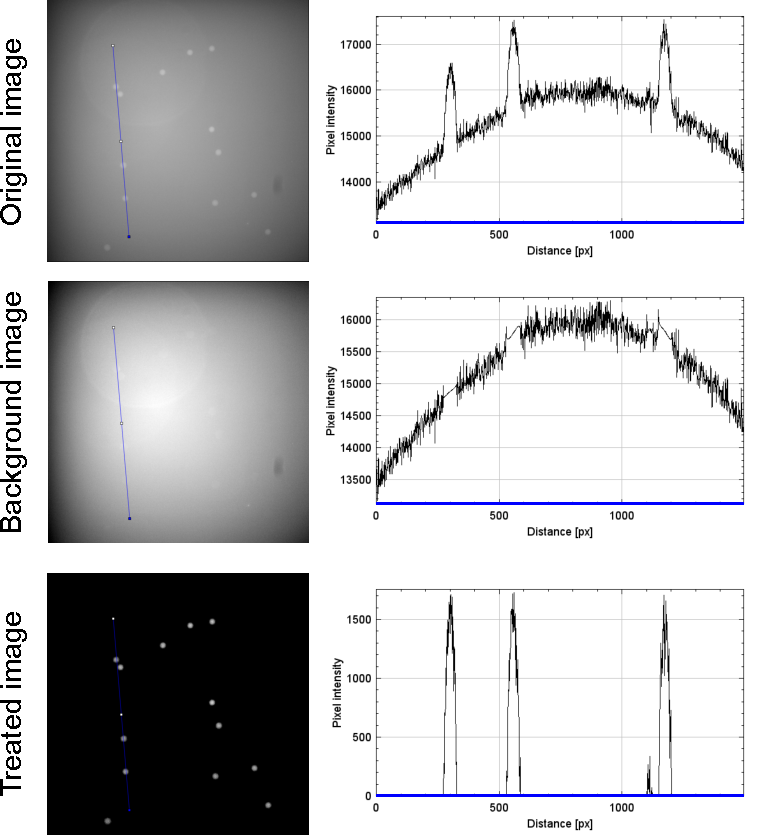
\includegraphics[scale=0.75]{fig11.pdf}
            \caption{Comparison of the saved images}
            \label{fig11}
    \end{figure}

    \item Now that we have finished the background substraction, we turn to the quantification of the beads. For each image, we go bead by bead as identified in the bead mask (figure \ref{fig6}). We then integrate the fluorescence signal of the treated image in each bead region. This yields an integrated fluorescence value per bead. We do this for every bead per image, and then proceed on every image per filter. We also extract the radius of each bead region, defined as the radius of region in the bead mask. All the bead radii and integrated intensities computed at this step are saved in a \verb|.csv| file.
    \item Finally, we pool all the results across images for a given condition and plot histograms for the bead radii and integrated fluorescence intensity. We indicate with a red line the median values in both plots, and the number of detected beads $n_\text{beads}$ (i.e., the number of regions in the bead mask). This is done for all filters. Figure \ref{fig12} shows the resulting histograms.
    
    \begin{figure}[H]
            \center
            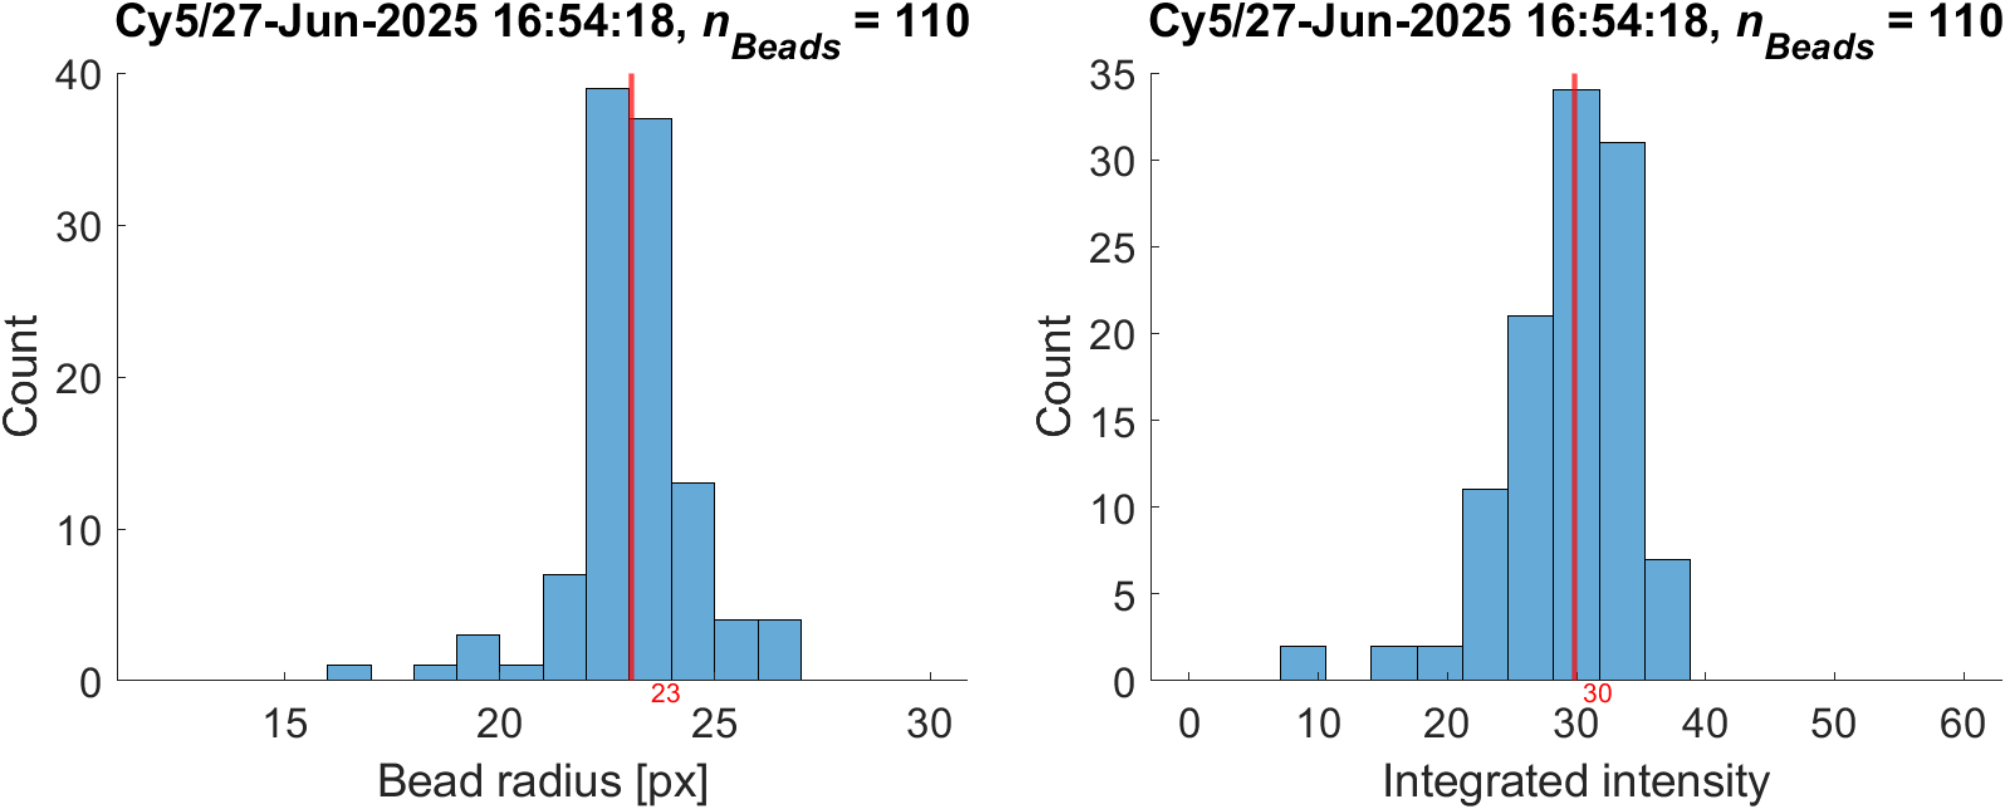
\includegraphics[scale=0.8]{fig12.png}
            \caption{Bead radius and integrated intensity histograms}
            \label{fig12}
    \end{figure}

\end{enumerate}
\end{document}